\documentclass{beamer}
\usepackage[italian]{babel}
\usepackage{graphicx}
\usepackage{bm}
\usepackage{hyperref}
\usepackage{hyperref}
\usepackage[italian]{babel}
\RequirePackage{palatino}
\RequirePackage[utf8]{inputenc}
\RequirePackage[T1]{fontenc}

\usefonttheme{serif}
\graphicspath{ {./pic/} }

\newcommand{\makepart}[1]{ % For convenience
\part{#1} \frame{\partpage}
}
\usepackage{styles/elegantmacros}
\usepackage{styles/bussproofs}
\usefolder{styles}
\usetheme[style=blue]{elegant}


\setlength{\itemsep}{50.mm}


\title[
]{Da Matita a Dedukti e ritorno}

\subtitle{sottotitolo che non so ancora cosa}

\author[
]{
    Mattia Girolimetto
}

\institute{
Relazione per il corso 85001 - Metodi logici per la Filosofia \\
    Alma Mater Studiorum, Università di Bologna}
\date{\today}

\begin{document}
\begin{frame}
  \titlepage
\end{frame}

\begin{frame}{Indice}
  \tableofcontents
\end{frame}

\section{I proof assistant}
\begin{frame}
\begin{center}

\includegraphics[scale=0.70]{coq.png}
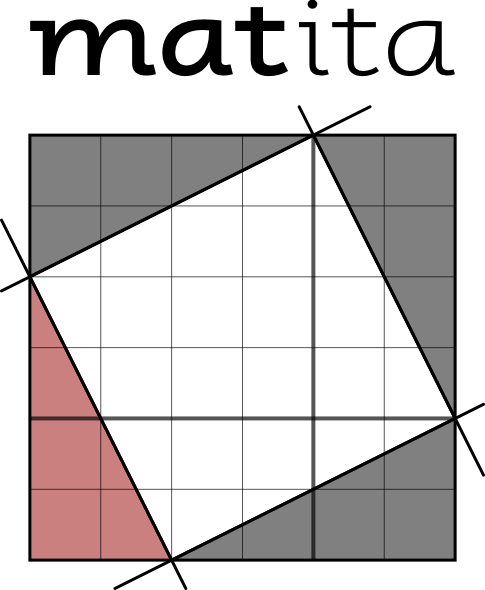
\includegraphics[scale=0.30]{matita.png}
\end{center}
\begin{center}
% 
\includegraphics[scale=0.30]{agda.png}
\end{center}
\end{frame}
\begin{frame}{Isomorfismo}
\end{frame}


\section{Dedukti}
\begin{frame}
\begin{columns}

\begin{column}{.5\textwidth}
\begin{itemize}
  \item Framework logico
  \vspace{1.5em}
  \item Implementa logiche e teoremi
  \vspace{1.5em}
  \item Basato sul $\lambda\Pi$-calcolo modulo
\end{itemize}
\end{column}

\begin{column}{.5\textwidth}

\includegraphics[scale=1]{dedukti2.png}
\begin{center}
    \href{https://deducteam.github.io/}{https://deducteam.github.io/}
\end{center}
\end{column}
\end{columns}


\end{frame}

\section{Matita}
\begin{frame}
\begin{columns}
  \begin{column}{.5\textwidth}
    \begin{itemize}
      \item Proof assistant sviluppato all'Università di Bologna
      \vspace{1.5em}
      \item Basato sul calcolo delle \textit{costruzioni (co)induttive}
    \end{itemize}
  \end{column}
  \begin{column}{.5\textwidth}
    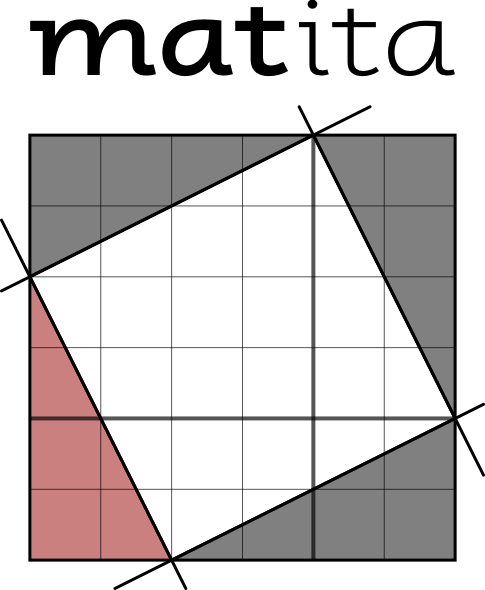
\includegraphics[scale=0.30]{matita.png}
  \href{https://github.com/sacerdot/matita}{https://github.com/sacerdot/matita}
  \end{column}
\end{columns}
\end{frame}

\section{Krajono}
\begin{frame}

\begin{columns}
\begin{column}{.5\textwidth}
\begin{itemize}
  \item \textit{Fork } di Matita 
  \vspace{1.5em}
  \item Esportazione verso Dedukti
  \vspace{1.5em}
  \item Non più supportato
\end{itemize}
\end{column}
\begin{column}{.5\textwidth}

\includegraphics[scale=0.40]{m2d.png}
  \href{https://github.com/Deducteam/Krajono}{https://github.com/Deducteam/Krajono}
\end{column}
\end{columns}

\end{frame}

\section{Esportazione}
\begin{frame}
  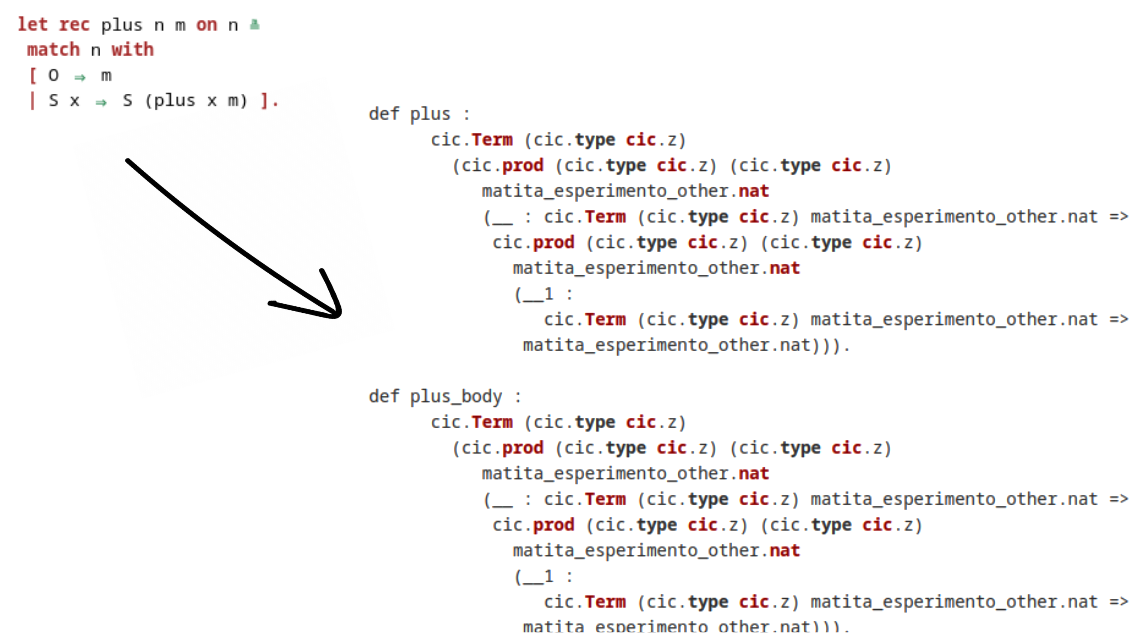
\includegraphics[scale=0.30]{export.png}
\end{frame}

\section{Importazione}
\begin{frame}

\end{frame}

\section{Le pragma}
\begin{frame}
\begin{itemize}
  \item \alert{\textbf{Problema}} Durante la codifica vengono perse informazioni necessarie
    alla ricostruzione dei termini originali.
  \vspace{1em}
  \item \alert{\textbf{Soluzione}} Preservare tali informazioni usando le \textit{pragma}.
\end{itemize}
  \vspace{3em}
  \begin{exampleblock}{Esempio}
\begin{center}
  \textbf{\texttt{\#PRAMGA BEGIN INDUCTIVE NAME=nat CONS:nat=O CONS:nat=S}}
\end{center}
  \end{exampleblock}
\end{frame}

\begin{frame}

\end{frame}

\section{Conclusioni}
\begin{frame}
\end{frame}

\end{document}
